%\mychapter{3}{methodology}

\section{Current Project}

\subsection{Our framework}

We propose a method of pre-procesing spike times by looking at the time since the 
last spike (previous time), smoothing the previous time using the Laplace kernel
and then using the diffusion distance \cite{coifman2006diffusion} as a measure of similarity
between spike trains. The low dimensional model is obtained by non-linear dimensionality reduction using the diffusion maps algorithm. The measure of ``goodness" of our low dimensional model is done by comparing the mutual information  \cite{quiroga2009extracting, Dayan2001}  between the resultant eigen vectors and and the position of the animal. We test our results using both simulations and behavioral real-world data.\\

A mathematical model based on the point-process framework is the best approach for 
modeling  data from the CA1 region of the rat hippocampus for two reasons.
First, the position of the animal is coded by place cells using both the firing rate
and the precise time at which the cells fire with respect to the hippocampal theta rhythm.
The theta rhythm is a sinusoid of frequency 7-12 Hz which occurs whenever a rat changes
position in  a specific direction \cite{OKeefe1971, Burgess1993}.
Second,  metrics based on the point-process viewpoint are often non-Euclidean \cite{Aronov2004, Victor2005}. Moreover, there are specific examples like sensory space in  the olfactory system and the perceptual space of color vision which are typically non-Euclidean and analysis in the point-process framework would be most appropriate.\\


\subsection{Nature of our Raw real-world data}
The raw data provided by the Redish Lab is a set of multiple single-unit single-trial
spike trains 
T = $\displaystyle \Set{ \{ t_{i}^{j} \} , 1 \leq i \leq n_{i}, 1 \leq j \leq 32 } $ 
recorded from 32 neurons called  place cells  in the CA1 region of the rat hippocampus.
$\displaystyle  \{t_{i}^{j}\} =  \{t_{1}^{j}, ....., t_{n_{i}}^{j} \} $ represents 
a sequences of n$_{i}$ recorded times at which the spikes of the j$^{th}$ neuron occurred.
The spike trains are of different lengths where t$_{i}^{j}$ represents the i$^{th}$
spike time of the j$^{th}$ neuron.

\subsection{Preprocessing raw spike train data}
We preprocessed the raw spikes using two methods.
In the first method, the raw spikes were smoothed with a Gaussian kernel to obtain a firing rate. In the second method, we computed the time since the last spike which we call the \textit{previous time}, and then smoothed the previous time with the Laplace Kernel.\\


\subsection{Conversation to a firing rate}
For each neuron labeled j,  we converted the corresponding spike train 
T$^{j}(t) = \displaystyle \sum_{i=1}^{n_{i}} \delta(t-t_{i}^{j}) $ into a firing rate,
 R$^{j}$(t) by replacing K in \eqref{firerate} with the  Gaussian Kernel\\
 K(t) =  $\displaystyle \frac{1}{\sigma \sqrt{2\pi}} e^{-\frac{t^2}{2\sigma^2}} $.
Thus, the firing rate for the j$^{th}$ neuron is given by

\begin{equation} \label{jfirerate}
R^{j}(t) = \sum_{i=1}^{n_{i}}  \frac{1}{\sigma \sqrt{2\pi}} 
e^{-\dfrac{(t_{i_{k}}^{j}  - t_{i_{l}}^{j})^2}{2\sigma^2}} 
\end{equation}

\subsection{Computing the previous time}
Let $\vect{s} = (s_1, s_2, ..., s_n)$  be a vector of n time points representing the different states of the animal's brain  where  $s_1 < s_2 < ... < s_n$. We  define the \textit{previous time} of the j$^{th}$ neuron at the $s_{k}$-th brain state  denoted by , p$^{j}(s_{k})$, as follows:\\
Let t$_{\max}$ = $\max  \Set{ t^{j}_{i} | t^{j}_{i} < s_{k},
1 \leq k \leq n \quad \text{for all} \quad  t^{j}_{i} }.$ Then p$^{j}(s_{k})$ = t$_{\max} - s_{k}.$\\
See example  \eqref{ex1} below.


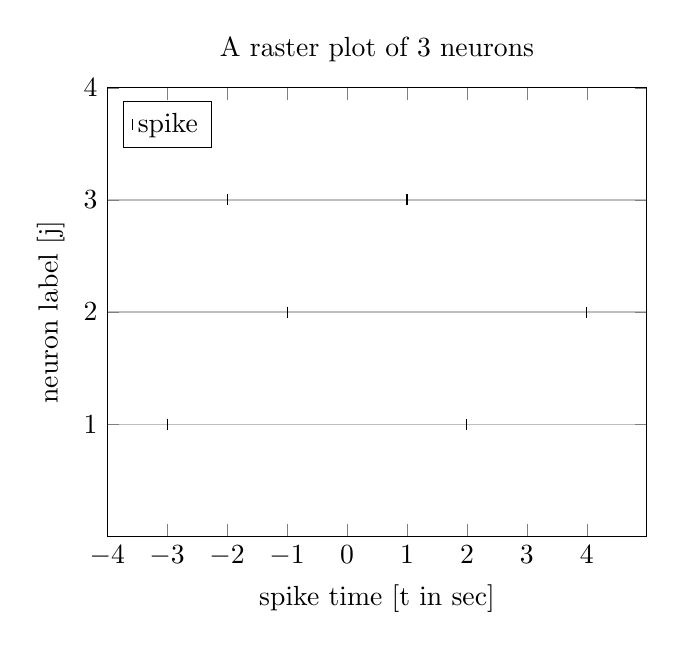
\begin{tikzpicture}
\begin{axis}[
    title={A raster plot of 3 neurons},
    xlabel={spike time [t in sec]},
    ylabel={neuron label [j]},
    xmin=-4, xmax=5,
    ymin=0, ymax= 4,
    xtick={-4, -3,-2,-1,0,1,2,3,4},
    ytick={1,2,3,4},
    legend pos=north west,
    ymajorgrids=true,
    grid style= solid,
]
 
\addplot[
    color=black,
    only marks,
    mark = |
    ]
    coordinates {
    (-3, 1)(-1,2)(-2, 3)(1, 3)(2,1)(4,2)
    };
    \legend{spike}
 
\end{axis}
\end{tikzpicture}


\begin{Ex}\label{ex1}
 \begin{align*}
    p^{j}(s_k=0) &= \begin{bmatrix}
           -3\quad \text{if} \quad j=1 \\
           -1\quad \text{if} \quad j=2\\
           -2\quad  \text{if} \quad  j=3
         \end{bmatrix},
  \end{align*} 
  
  \quad
  
  \begin{align*}
    p^{j}(s_k=2) &= \begin{bmatrix}
           -5\quad \text{if} \quad j=1 \\
           -3\quad \text{if} \quad j=2\\
           -1\quad  \text{if} \quad  j=3
         \end{bmatrix}
  \end{align*} 
  
\end{Ex}


\subsection{Specific implementation}

\subsubsection{Our distance measures}

\subsubsection{Our similarity measures}

\subsubsection{Place field model}

\subsubsection{Firing rate simulation}

\subsubsection{Previous time approach}

\subsubsection{Initial Results}

\subsubsection{Modification}




\newpage





















%\begin{itemize}

%========suggested by Duane=========================================
%\item  First mention that there is a general conceptual framework
%namely dimensionality reduction and then say that
% the metric a approach is just one of the ways of doing dim reduction
% yet ensuring minimal information loss.

%\item The previous/next time approach is our new way of preprocessing
% the data and then using some of the usual metrics to analyze it.

%============end suggestion=========================================
%\item How did you create the metric and what precisely is it's definition?
%\item Experimental design. Discuss how the data was collected using a diagram
%\item Mention that this kind of analysis has never been 
%applied to this Redish Lab data.
%\item describe your methodology starting with the fake brain model and then tests on real data
%\item what are the names and definitions of the algorithms you're using?
%\item what is dimensionality reductions and why are you using linear instead of non linear
%\item Why did you choose this particular algorithm(s)?
%\item What is wrong with using PCA or Kernel PCA?
%
%\end{itemize}





